\subsection{What our design can and cannot establish}
\label{discussion:design}

Two methodological points are worth stating explicitly, because they define
the boundary of what this analysis can claim.

First, several exhibits in this report -- most notably the covariate-balance
comparison in Section~\ref{data:balance} -- compare the distribution of a
variable (assets, gender, and so on) \emph{conditional on} compensation
group, rather than modelling compensation status as an outcome to be
predicted from those variables. This is a deliberate choice, not an
oversight: its purpose is to check whether the two compensation groups are
comparable before any later comparison is trusted, exactly as a baseline
characteristics table does in an observational or quasi-experimental study.
The complementary, predictive-direction question -- do these same variables
predict who applies for compensation? -- is answered separately, inside the
main structural model itself (Section~\ref{model:spec}), where
sociodemographic and background constructs have explicit paths \emph{to}
compensation participation. There, only household income reaches
significance ($\beta = 0.080$, $p = .047$); gender is borderline
($\beta = 0.069$, $p = .060$); age, education, and household assets are not
significant predictors of compensation participation once the other
background variables are accounted for jointly. Both directions of analysis
appear somewhere in this report; neither substitutes for the other.

Second, every coefficient in this report is an \emph{association}, adjusted
for the other variables in the same model, not a causal effect. The data are
observational and cross-sectional: compensation status was not randomly
assigned, and we do not observe tolerance before a household applied for
compensation. Where we write that compensation participation is "negatively
associated with" tolerance, we mean precisely that and no more.

\subsection{Sensitivity checks on the main finding}
\label{discussion:sensitivity}

We ran three further checks aimed at the most likely ways in which the
compensation paradox could be an artefact. All three are exploratory and
were added after the main analysis; they use ordinary regression on the
construct scores from the main model, or a separate latent-variable model,
and are reported here to qualify the main result, not to replace it.

\paragraph{Does the association hold within each county?} Compensation
status is strongly tied to county (Section~\ref{data:confound}), and with
only two counties a site covariate cannot fully separate the two. We
therefore re-estimated the compensation--tolerance association separately
in each county (Table~\ref{tab:within-county}). The association is negative
in both. In Qingchuan it is clearly different from zero. In Baoxing the
point estimate is, if anything, larger, but the confidence interval is wide
and includes zero: only 41 of the 160 Baoxing respondents did not apply for
compensation, so that comparison is imprecise. A formal
compensation~$\times$~county interaction is not significant ($p = .34$). The
paradox is therefore not produced by pooling two different counties, but the
statistical evidence for it rests mainly on Qingchuan.

\begin{figure}[htbp]
\centering
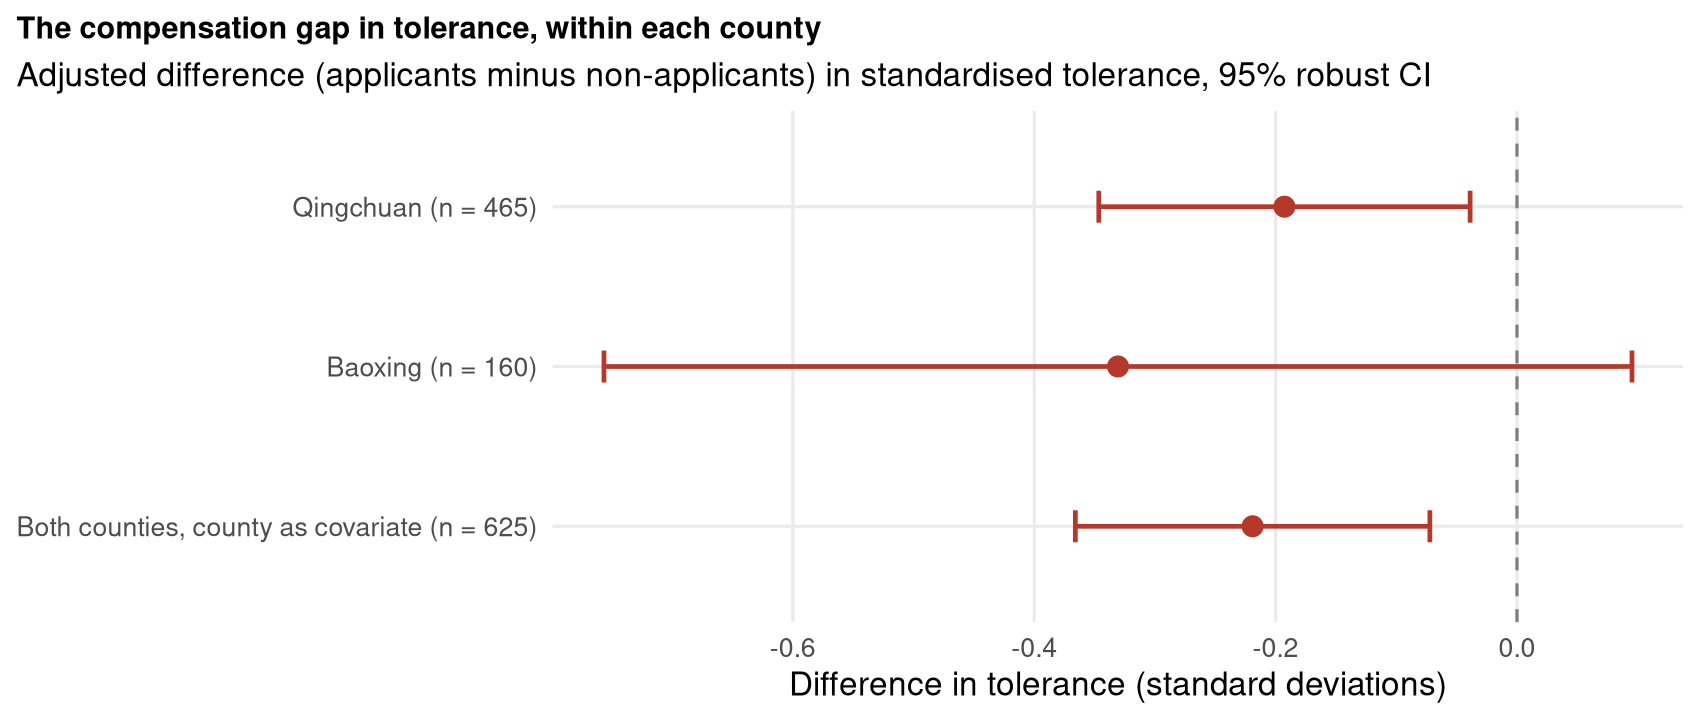
\includegraphics[width=0.9\textwidth]{figures/fig_within_county.png}
\caption{The adjusted compensation gap in tolerance, in each county and with
both counties pooled.}
\label{fig:within-county}
\end{figure}

\begin{table}[htbp]
\centering
\caption{Compensation participation and tolerance within each county.
Entries are the adjusted difference in the standardised tolerance score
between applicants and non-applicants (in standard deviations), from a
linear regression on the construct scores of the main model, controlling
for the background variables and the mediator constructs, with
heteroscedasticity-robust (HC3) standard errors. Because compensation
participation is entered as a 0/1 variable here, these values are on a
different scale from the standardised $\beta$ in Table~\ref{tab:rq1}.}
\label{tab:within-county}
\begin{tabular}{lrrrr}
\hline
\textbf{County} & \textbf{$n$} & \textbf{Difference} & \textbf{95\% CI} & \textbf{$p$} \\
\hline
Qingchuan & 465 & $-0.19$ & $[-0.35,\ -0.04]$ & .014 \\
Baoxing   & 160 & $-0.33$ & $[-0.76,\ 0.10]$  & .127 \\
Pooled, with county as covariate & 625 & $-0.22$ & $[-0.37,\ -0.07]$ & .004 \\
\hline
\end{tabular}
\end{table}

\paragraph{Could measurement error hide a mediator?} Our mediators are short
self-report blocks. Random measurement error in a mediator has two known
consequences, which is why it is a natural suspect for ``missing'' mediation.
First, it causes \emph{attenuation bias}: the estimated effect of the
mediator on tolerance (the second leg) is pulled towards zero, and with it
the indirect effect, which is the product of the two legs. Second, it causes
\emph{incomplete adjustment}: because compensation participation is
correlated with the mediator, part of the mediator's true influence is not
absorbed by the noisy measure and shows up instead as a direct effect of
compensation. Together these can make a truly mediated effect look direct.
PLS-SEM composites do not correct for either problem.

As a sensitivity analysis we refitted the model as a latent-variable model
(R package \texttt{lavaan}, WLSMV estimator), with tolerance as an ordinal
latent factor and \emph{all five} mediators entered together, each as a latent
variable measured by its construct score with an assumed reliability between
1.0 (no error) and 0.6 (Table~\ref{tab:latent}). The same reliability was
applied to every mediator because we have no external estimate for each one.
For the formative constructs, whose indicators are not assumed to be
error-free copies of one quantity, this is a sensitivity assumption, not an
estimated property, and the results should be read in that light.

The result is the same at every assumed reliability. Correcting for error
strengthens the second leg for intangible cost considerably (standardised
path $-0.41$ without correction, $-0.65$ at reliability 0.6) and the
indirect effect through intangible cost grows from $-0.021$ to $-0.044$, but
its interval always includes zero. The indirect effects through the other four
mediators stay close to zero, as does the total indirect effect
($-0.032$ to $-0.049$, intervals including zero throughout), and the direct
association between compensation and tolerance stays negative and different from
zero ($-0.146$ to $-0.129$). The limiting factor is the first leg. Random
error in a mediator that serves as an \emph{outcome} of compensation does not
bias that first-leg coefficient; it only widens its interval. Compensation
participation is barely related to intangible cost ($+0.05$ to $+0.07$,
$p \approx .22$) or intangible benefit ($-0.04$ to $-0.05$, $p = .35$), and
no correction for random error can create a relationship that is not there.
The two mediators with a nominally detectable first leg, compensation anticipation
($+0.09$ to $+0.12$, $p \approx .04$) and, borderline, tangible cost, have a
second leg indistinguishable from zero ($-0.03$ and $+0.02$ to $+0.14$).
We conclude that attenuation from random measurement error does not explain
the absence of mediation in this data. Two other kinds of error are not
covered by this analysis and could work in the opposite direction: error that is
shared between intangible cost and tolerance because both are reported by the
same person (which would inflate their second leg, see
Section~\ref{discussion:limitations}), and error that depends on compensation
status itself (differential error), for instance if applicants rate costs
differently because of their dealings with the compensation process.

\begin{table}[htbp]
\centering
\caption{Latent-variable sensitivity analysis for all five mediators:
standardised indirect effects of compensation participation on tolerance
(95\% CI in brackets) under different assumed reliabilities of the mediator
scores. CA: compensation anticipation; PS: policy support; TC: tangible cost;
IC: intangible cost; IB: intangible benefit. Direct is the compensation
$\rightarrow$ tolerance path. Values are comparable across rows, but not in
size with the PLS-SEM coefficients in Table~\ref{tab:rq1}.}
\label{tab:latent}
\small
\begin{tabular}{crrrrrrr}
\hline
\textbf{Rel.} & \textbf{Direct} & \textbf{via CA} & \textbf{via PS} & \textbf{via TC} & \textbf{via IC} & \textbf{via IB} & \textbf{Total indirect} \\
\hline
1.0 & $-0.15$ & $-0.003$ & $-0.002$ & $+0.001$ & $-0.021$ & $-0.008$ & $-0.032\ [-0.075,\ 0.010]$ \\
0.9 & $-0.14$ & $-0.003$ & $-0.002$ & $+0.002$ & $-0.024$ & $-0.009$ & $-0.035\ [-0.083,\ 0.012]$ \\
0.8 & $-0.14$ & $-0.003$ & $-0.002$ & $+0.004$ & $-0.028$ & $-0.009$ & $-0.039\ [-0.094,\ 0.015]$ \\
0.7 & $-0.13$ & $-0.004$ & $-0.002$ & $+0.007$ & $-0.034$ & $-0.010$ & $-0.044\ [-0.108,\ 0.021]$ \\
0.6 & $-0.13$ & $-0.005$ & $-0.002$ & $+0.013$ & $-0.044$ & $-0.011$ & $-0.049\ [-0.129,\ 0.031]$ \\
\hline
\end{tabular}

\smallskip
\footnotesize The 95\% interval of every individual indirect effect includes zero at all
reliabilities; the direct path is significant ($p < .03$) at all reliabilities.
\end{table}

\paragraph{What the robustness analysis does and does not show.} That the
compensation coefficient is negative in all 8{,}192 specifications
(Section~\ref{robustness}) shows that the result does not depend on our
analytic choices. It does not show that the association is causal, or free
of bias: every specification uses the same respondents, the same
self-reported measures, and the same non-random assignment to compensation,
so any bias from those sources is present in all of them.

\subsection{Limitations}
\label{discussion:limitations}

Five limitations bound every conclusion in this report. First, the
comparison is cross-sectional: we lack each respondent's tolerance before
they applied for compensation, and payment timelines are not consistently
established across respondents, so we cannot rule out that some of the
association we attribute to compensation participation reflects
pre-existing differences between residents who chose to apply and those who
did not. Second, county and survey period coincide completely
(Section~\ref{data:confound}), and the sampling frame and any exclusions
applied before we received the data are incompletely documented; we have
controlled for the county/survey-wave confound statistically, but cannot
rule out other, unrecorded differences between the two fieldwork rounds.
Third, several measurement blocks are short and conceptually overlapping
(Section~\ref{measurement:formative}), and the free-text word responses
used for part of the intangible-cost measure have structural missingness;
together these limit how strongly we can claim to have isolated distinct
latent psychological constructs, as opposed to correlated but imperfectly
separated ones. Fourth, tolerance and intangible cost are both attitudes
reported by the same person in the same interview. A respondent who is
generally aggrieved is likely to rate wild boar more negatively and to
report lower tolerance at once, so part of the strong intangible
cost--tolerance association may reflect shared reporting tendencies rather
than one attitude driving the other; the discriminant-validity result in
Section~\ref{measurement:formative} points the same way. The finding that
intangible cost is the strongest correlate of tolerance should be read with
this in mind. Fifth, tolerance itself is measured with limited reliability
(Section~\ref{measurement:efa-cfa}), and the mediation, moderation, and
multi-group analyses involve many tests on one data set. We treat the
compensation--tolerance path as the one confirmatory result; the mediation
and moderation results are mostly null findings, for which the sample gives
limited power (Section~\ref{model:rq1}), and the single multi-group
difference we report should be regarded as exploratory until replicated.

\subsection{Recommendations for the next study}
\label{discussion:next-steps}

Three concrete steps would materially strengthen the next round of analysis
or data collection. First, several fieldwork details should be clarified
directly with the project partner before any further modelling: the exact
routing between applying for and receiving compensation, which sampling
exclusions were applied and why, precise fieldwork dates, the units
underlying the area variables, and the small number of compensation-
percentage responses that exceed 100\% of assessed loss
(Section~\ref{data:quality}). Second, once those clarifications are in hand,
the report should be revised transparently, re-running only the specific
analyses that those clarifications affect, rather than the full pipeline,
so that the provenance of every number remains traceable. Third, and most
importantly for RQ1, a future panel study should measure tolerance and
related attitudes \emph{before} a household applies for compensation and
again \emph{after} payment is received, with a clearer set of indicators and
an explicit comparison design. Only a before/after design of this kind can
distinguish whether compensation genuinely lowers tolerance, whether
lower-tolerance households are simply more likely to apply in the first
place, or whether both are downstream of some third factor -- such as prior
conflict severity or grievance with the compensation process itself -- that
the present cross-sectional survey cannot measure.
